\documentclass{article}

\author{phunc20}
\title{Integer Addition in C}

\usepackage{tikz}
\usepackage{graphicx}
\usepackage{amsmath}
\usepackage[utf8]{vietnam}

%\usepackage{pgfplots}
%\usepgfplotslibrary{polar}

\begin{document}
\maketitle
Trong bài này mình sẽ nói về cách cộng/trừ (\texttt{+}/\texttt{-}) \texttt{int}'s trong ngôn ngữ C. Cái mà được trình bài ở đây chỉ là những gì mình hình dung được, có thể có sai sốt; mình cũng đang trên đường học tập; nếu bạn đọc nào tìm ra những chỗ bị sai, có thể liên lạc với mình bằng email.

\section{Cách biểu thị \texttt{int}}
Để dễ cho việc thảo luận, mình sẽ coi \texttt{int} như luôn được lưu và xử lý trong máy tính bằng 32 bits. Hơn nữa, binary và decimal integers sẽ được biểu thị như, e.g. số bảy, $(111)_{2} = (0\cdots0111)_{2}$ và $7$, resp.

Thử giả bộ chúng ta là những người đầu tiên chuẩn bị chế ra tiêu chuẩn cho \texttt{int}.
Một cách tự nhiên, mình quy định $(0\cdots0)_{2} = 0, (0\cdots01)_{2} = 1, (0\cdots010)_{2} = 2, (0\cdots011)_{2} = 3$, etc. Cái này cho đến khi $(01\cdots1)_{2} = 2^{31} - 1$. Mình tạm dừng ở đây là tại vì (\romannumeral 1) đến đây mình đã cho hết một nửa các con số 32-bit; (\romannumeral 2) mình còn chưa assign số âm nào hết.
\subsection{Chế tậm bậy}
Các con số 32-bit còn lại, thật ra mình cũng có quyền chế tùy ý. Ví dụ như, 
$$-1 = (10\cdots01)_{2}, -2 = (10\cdots010)_{2},\;\ldots, -(2^{31} - 1) = (1\cdots1)_{2}.$$

Và cái con số 32-bit cuối cùng sao cũng được:
$$(10\cdots0)_{2} = 2^{31} \;\textrm{hoặc}\; (10\cdots0)_{2} = -2^{31}.$$
\vfil \break

\subsection{Chế đằng hoàng}
Thật ra, không có ai bắt con người mình chế tiêu chuẩn cho \texttt{int} nhất quyết phải như thế nào cả. Điều quan trọng ở đây là \textit{một tiêu chuẩn được chế ra và sử dụng rộng rãi vì sự thuận thiện nó măng lại}.

Cái tiêu chuẩn mà mình chế đại ở section trước, nó \textbf{tiện ở chỗ} là dễ nhận ra con số đó là bao nhiêu (tại vì số dương và số âm chẳng khác gì ngoài bit đầu tiên). Nhưng mà nó lại \textbf{bất tiện ở chỗ}, chẳng hạn như $(-1) + 1$ sẽ là
$$(10\cdots01)_{2} + (0\cdots01)_{2}.$$
Rất khó để giải thích tại sao cái này tính ra $(0\cdots0)_{2}$.

Cái tiêu chuẩn những người đi trước mình chế ra, đó là
\begin{equation*}
\begin{split}
	&(10\cdots0)_{2} = -2^{31}, (10\cdots01)_{2} = -2^{31} + 1, (10\cdots010)_{2} = -2^{31} + 2, \;\ldots, \\
	&(1\cdots101)_{2} = -3, (1\cdots10)_{2} = -2, (1\cdots1)_{2} = -1.
\end{split}
\end{equation*}
Theo mình cách chế này \textbf{được cái tiện ở chỗ} cách cộng được tự nhiên và như \emph{group} trong toán học. Ví dụ:
\begin{itemize}
	\item $(10\cdots0001)_{2} + (00\cdots0011)_{2} = (10\cdots0100)_{2} = -2^{31} + 4$ on one side, and $(-2^{31} + 1) + 3 = -2^{31} + 4$ on the other;
	\item $(1\cdots1)_{2} + (0\cdots01)_{2} = (10\cdots0)_{2} \,(\textbf{một cái 1 và ba mươi hai cái 0}) = (0\cdots0)_{2} \,(\textbf{32 cái 0})$ ở một phía, và $(-2^{31} + 1) + 1 = 0$ ở phía còn lại.
\end{itemize}

Cái cách cộng hai \texttt{int}'s trong hệ thổng này giống Hình 1 ở dưới, khi tính \texttt{a + b} mình có thể đi từ \texttt{a} theo hướng kim đồng hồ số bước từ \textbf{số không} tới \texttt{b}; nếu cách cộng đó xoay hơn một vòng hình tròn thì mình tính lại từ đầu (i.e. từ \textbf{số không}). Các bạn đọc có thể lấy ba ví dụ hình dung trong đầu và verify có thật: (\romannumeral 1) cộng hai con số dương; (\romannumeral 2) một con số dương và một con số âm; (\romannumeral 3) hai con số âm.

\begin{figure}[h!]
  \centering
  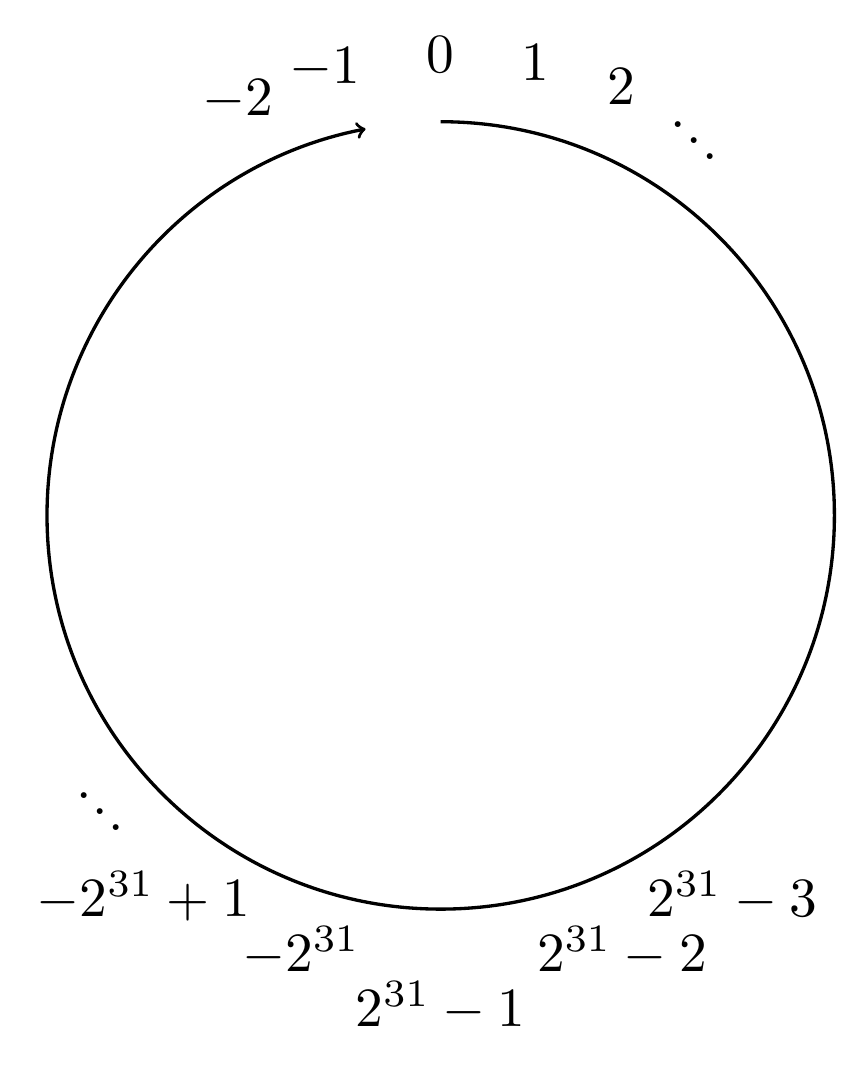
\begin{tikzpicture}
  	%\draw[->] (0,0) circle (5cm);  % -> doesn't work
  	\draw[very thick,->] (0,5) arc (90:-259:5cm);
  
  	% annotate the int
  	%\draw (0,5) node[anchor=south] {$\Large 0$};  % 0 too small
  	%\draw (0,5.5) node[anchor=south] {\scalebox{2}{$\Large 0$}};  % cf. https://tex.stackexchange.com/questions/3703/make-equations-large
  	\node[above]       at (0, 5.5) {\scalebox{2}{$0$}};
  	\node[above right] at (0.9, 5.4) {\scalebox{2}{$1$}};
  	\node[above right] at (2, 5.1) {\scalebox{2}{$2$}};
  	%\node[above right] at (3, 4.7) {\scalebox{2}{.}};
  	\node[above right] at (2.8, 4.8) {\scalebox{2}{.}};
  	%\node[above right] at (3.2, 4.6) {\scalebox{2}{.}};
  	\node[above right] at (3.0, 4.6) {\scalebox{2}{.}};
  	%\node[above right] at (3.4, 4.5) {\scalebox{2}{.}};
  	\node[above right] at (3.2, 4.4) {\scalebox{2}{.}};
  
  	\node[above left] at (-0.9, 5.3) {\scalebox{2}{$-1$}};
  	\node[above left] at (-2, 4.9) {\scalebox{2}{$-2$}};
  	%\begin{polaraxis}
  	%	\draw (4.8,10) -- (5.2,10);
  	%\end{polaraxis}
  
  	%\node[below]       at (0, -5.5) {\scalebox{2}{$127$}};
    \node[below]       at (0, -5.8) {\scalebox{2}{$2^{31}-1$}};
  	%\node[below right] at (0.9, -5.3) {\scalebox{2}{$126$}};
    \node[below right]  at (1.1, -5.1) {\scalebox{2}{$2^{31}-2$}};
  	%\node[below right] at (2.3, -4.8) {\scalebox{2}{$125$}};
    \node[below right] at (2.5, -4.4) {\scalebox{2}{$2^{31}-3$}};
  	%\node[below left] at (-0.9, -5.3) {\scalebox{2}{$-128$}};
    \node[below left] at (-0.9, -5.1) {\scalebox{2}{$-2^{31}$}};
  	%\node[below left] at (-2.3, -4.8) {\scalebox{2}{$-127$}};
    \node[below left] at (-2.3, -4.4) {\scalebox{2}{$-2^{31}+1$}};
  	\node[below left] at (-3.9, -3.8) {\scalebox{2}{.}};
  	\node[below left] at (-4.1, -3.6) {\scalebox{2}{.}};
  	\node[below left] at (-4.3, -3.4) {\scalebox{2}{.}};



  \end{tikzpicture}
	\vspace{1cm}
	\caption{Để cộng hai \texttt{int}'s trong C, chúng ta có thẻ coi như đi bao nhiêu bước trên hình tròn như trong hình.}
	%\caption{In C, the addition of any two \texttt{signed int} (here for example $8\,$-bit) is nothing more than a compound clockwise rotation along the circle}
  %\label{int_circle}
\end{figure}


Một hệ quả của cách chế này là
\begin{itemize}
	\item $(\textrm{bit bên tay trái nhất}=0) \implies$ số không âm (i.e. số dương hoặc số $0$) ;
	\item $(\textrm{bit bên tay trái nhất}=1) \implies$ số âm.
\end{itemize}

Due to the cyclic nature of the addition we just defined, khi mình có một \texttt{int a} và mình muốn tìm \texttt{-a}, mình sẽ tiến hành như sau:\\
Nhắc lại $$(10\cdots0)_{2} \,(\textbf{một cái 1 và ba mươi hai cái 0}) = (0\cdots0)_{2} \,(\textbf{ba mươi hai cái 0}).$$
Để tìm được \texttt{b} sao cho \texttt{a} đi thêm \texttt{b} bước theo chỉ kim đồng hồ tới $(10\cdots0)_{2} = 0$, mình có thể
\begin{itemize}
	\item tìm trước \texttt{c} sao cho $\texttt{a + c} = (1\cdots1)_{2} = -1$. Việc này có thể đơn giản hoàn tất bằng cách đổi ngược từng bit trong \texttt{a}
	\item rồi $\texttt{b} = \texttt{c} + 1$
\end{itemize}
%\thispagestyle{empty}

Bài này đến đây đã hơi hơi bị dài, nếu các bạn đọc cảm thấy hứng thú, sau đây là một vài hướng các bạn có thể tự suy nghĩ tiếp:
\begin{enumerate}
	\item chứng minh cách cộng này là \emph{commutative} và \emph{associative}
	\item $\texttt{a - b} := \texttt{a + (-b)}$ theo đúng sense mình hay nghĩ về cách trừ giữa \texttt{int}'s. (Hint: It might be easier to think of this geometrically: rotating the angle of \texttt{-b} \textbf{clockwise} is equiv. to rotating \textbf{counter-clockwise} the angle of \texttt{b})
\end{enumerate}

\end{document}
